\chapterimage{chapter_head_2.jpg} % Chapter heading image

\chapter{Accommodation}

The majority of New College graduate students are housed in College accommodation for their first year of graduate study with a reasonable chance of receiving second year housing. New College graduates receive some of the most desirable accommodation facilities that are provided for students living in Oxford. Graduate students are mainly housed together in the Weston buildings, with growing numbers of students living in Castle Mill and Warham House. All accommodation costs approximately \pounds130 per week.

All College-owned graduate rooms are single study bedrooms that have a wealth of facilities including desk spaces, lamps, bookshelves, internal telephone, Ethernet connection, and heaters. As of 2013, the buildings have also been fitted with wireless Internet access.  Rooms will have 240\,V electrical sockets as well as sockets for razors near the basins.

Graduate rooms are kept clean by the college scouts. The scouts tidy communal areas each weekday and thoroughly clean your room on a weekly basis. It is usual to tip your scout either at Christmas or when you leave at the end of the academic year. The scouts are an integral part of college life so please do not hesitate to introduce yourself when they come by. 

The college housing regulations state that graduates may invite guests to stay in their rooms, but only for a maximum of two nights at a time. Alternatively, students can book one of the JCR single or double guest rooms, which are available very cheaply. If you wish to book one of these rooms please contact the Home Bursar's secretary Joan Fraser (\href{mailto:joan.fraser@new.ox.ac.uk}{\urlformat{joan.fraser@new.ox.ac.uk}}), but arrange this well in advance since these rooms are very popular during each term.

\section{Weston Buildings}

The Weston Buildings are located alongside a branch of the River Cherwell at the 
College Sports Ground, which is a short seven-minute walk from the main college site. The buildings provide 96 rooms for graduate students, which are divided into 16 houses. The rooms are modern, have a sink, and are well proportioned. Each house has a large self-catered kitchen with a patio area, four toilets, and three shower rooms. Laundry facilities are located in a small building opposite House 16.

\section{Warham House}
Warham house has 9~rooms for first-year and returning graduate students. It is located on Mansfield Road about two minutes' walk from college. It has recently been refurbished to a very high standard. The rooms are mostly large, although they are all different. There are a couple of kitchens, five toilets and four bath/shower rooms. There is one washing machine and tumble dryer.

\section{Castle Mill}
Castle Mill is a university accommodation complex situated in
central west Oxford close to the Railway Station, which is a ten-minute bike ride from the college and many research buildings of
the University. Each of the newly constructed 18 bedrooms earmarked for New
College has en-suite bathroom facilities with a kitchen and dining room that is shared between
the four to six students on each floor. There are four washing machines and
dryers available on site.

\begin{figure}[htbp]
\centering
		\begin{minipage}{0.28\textwidth}
                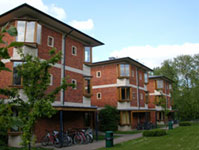
\includegraphics[width=\textwidth]{weston.jpg}
        \end{minipage}%
        \quad
        \begin{minipage}{0.28\textwidth}
                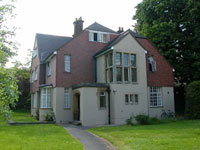
\includegraphics[width=\textwidth]{warham.jpg}
        \end{minipage}%
        \quad
        \begin{minipage}{0.35\textwidth}      
                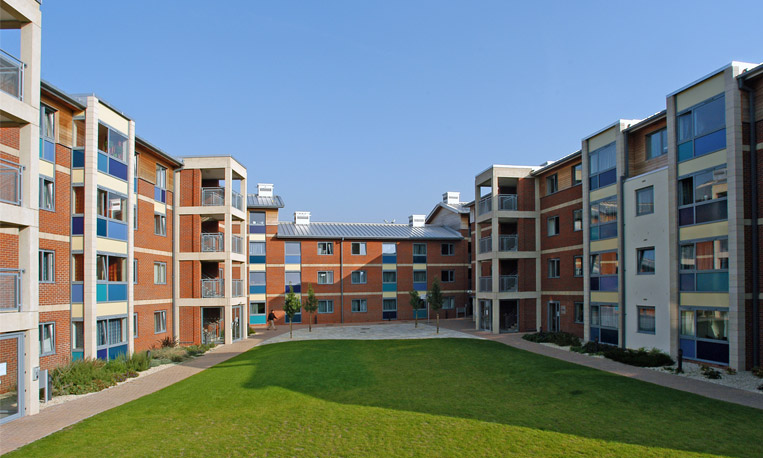
\includegraphics[width= \textwidth]{castlemill.jpg}
        \end{minipage}%
        \caption[]{The Weston complex,
        Warham house and Castle Mill accommodation sites.}
        \label{fig:accomm}
\end{figure}

\begin{figure}[htbp]
\centering
		\begin{minipage}{0.50\textwidth}
                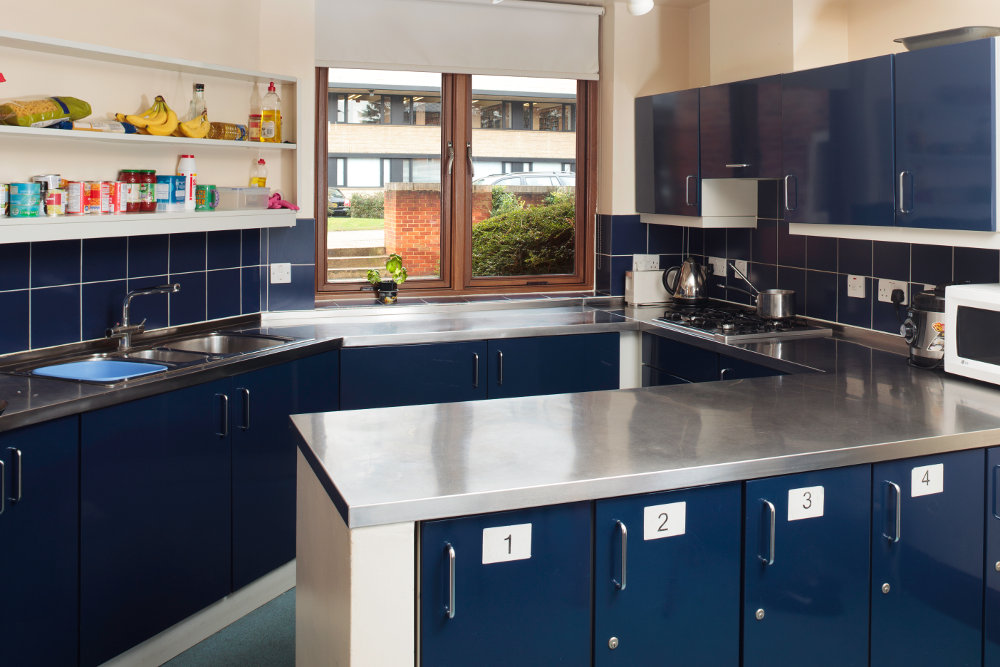
\includegraphics[width=\textwidth]{kitchen.jpg}
        \end{minipage}%
        \quad
        \begin{minipage}{0.46\textwidth}
                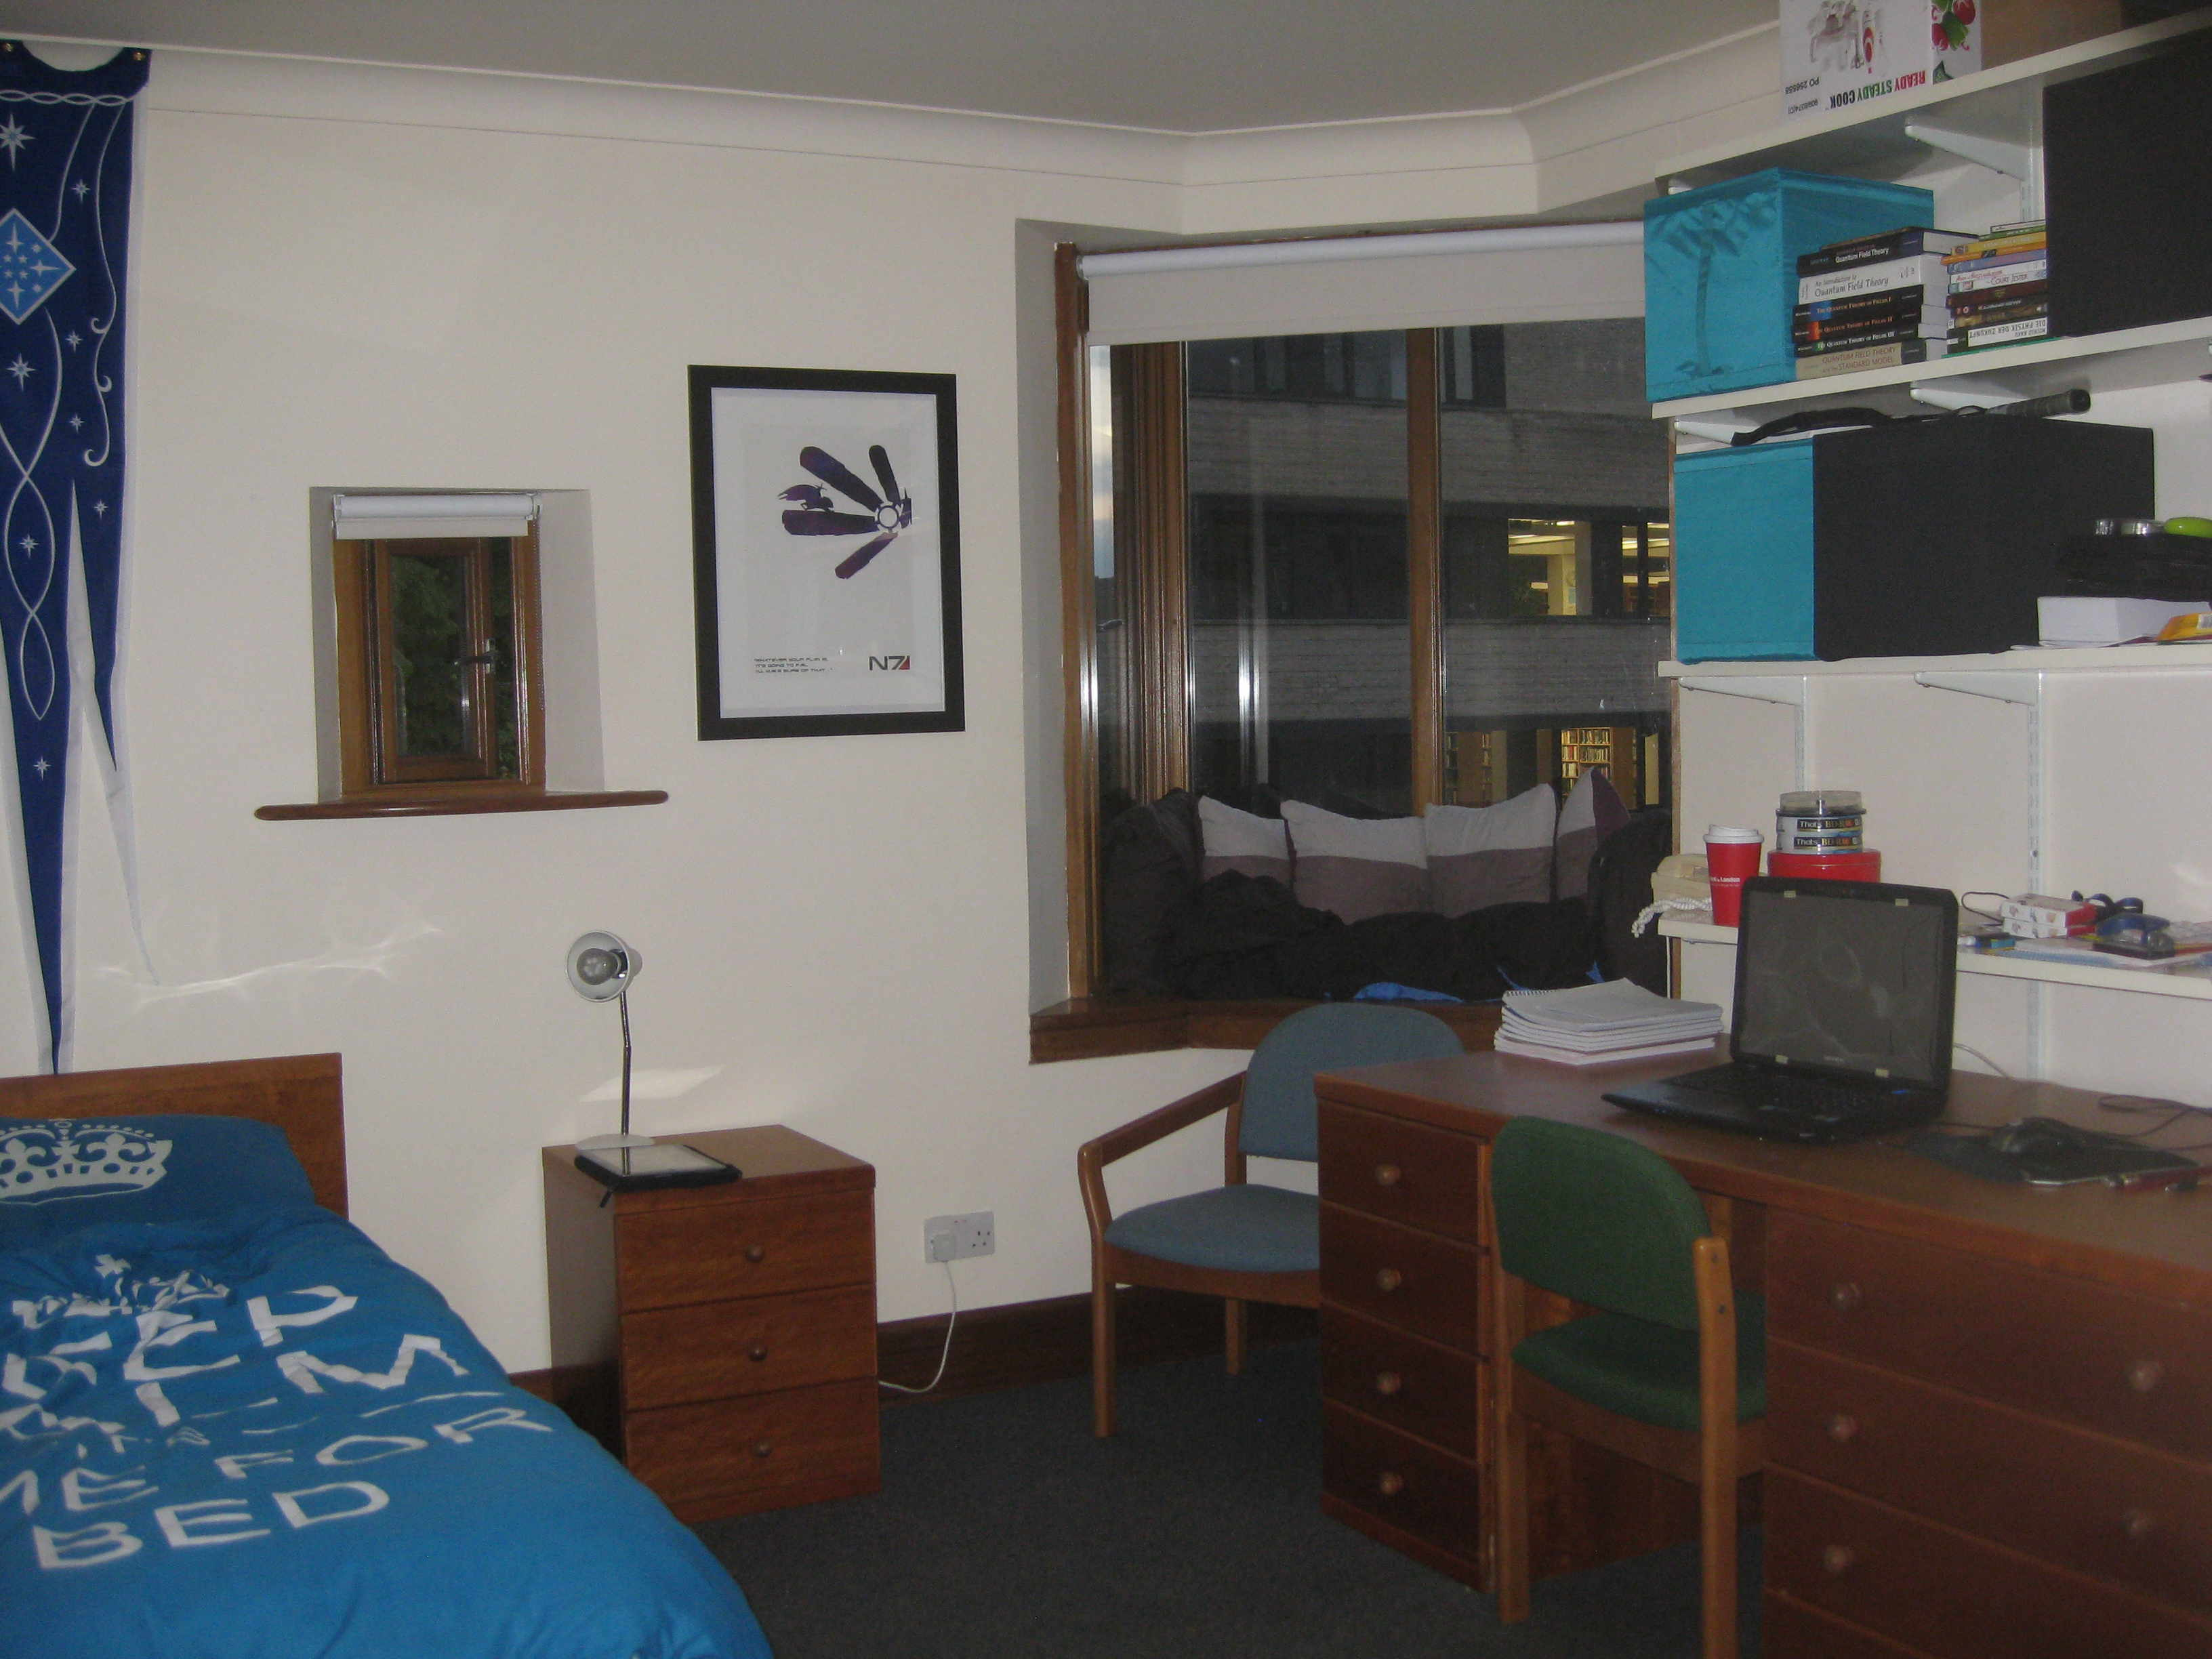
\includegraphics[width=\textwidth]{weston2.jpg}
        \end{minipage}%
\caption[]{A kitchen and a typical room
in the Weston buildings}
\label{fig:weston}
\end{figure}



